\documentclass[11pt]{article}

\usepackage[utf8]{inputenc}
\usepackage[a4paper, margin=1in]{geometry}
\usepackage{cite}
\usepackage{anyfontsize}
\usepackage{graphicx}
\usepackage{tabularx}

\title{Voice Recorder}
\author{sumanasekarawkgg.19 }
\date{\today}

\begin{document}
%\maketitle
\thispagestyle{empty}
\begin{center}
   
   \begin{figure}
   \vspace*{1.5cm}
       \centering
       
\includegraphics[width=4.8cm]{Images/uom.png}
   \end{figure}
   
   Department of Electronic and Telecommunication Engineering \\ University of Moratuwa \\
   \vspace{2cm}
   {\fontsize{14}{17}\selectfont\textbf{\\Simple Voice Recorder\\}}
    \vspace{6cm}
   \begin{tabularx}{0.5\textwidth}{ 
  >{\raggedright}X 
  >{\raggedright}}
     Silva G.B.N.M. & 190592X \\ 
     Siriwardana H.M.P. & 190595J \\  
     Sumanasekara W.K.G.G. & 190610E \\
     Thanushan K. & 190621M 
   \end{tabularx}
   \vspace{1cm}
   \\Supervisor: Mr. Thamindu Pathirana 
   \vspace{2cm}
   \\This report is submitted as a partial fulfilment of module EN1093
   \vspace{0.5cm}
   \\15 August 2021
\end{center}
%table of content
\newpage
\thispagestyle{empty}
\tableofcontents
%report start
\newpage
\twocolumn
\clearpage
\pagenumbering{arabic} 
\addcontentsline{toc}{section}{Abstract}
\section*{Abstract}
{\fontsize{10}{12}\selectfont\textbf{The project given to our group was to build a simple voice recorder that records audio files, saves them in a SD card and plays them when required. Also, the project had a requirement of adding an effect that makes a change in the frequency spectrum of the audio file. Softwares such as Arduino and AVR were used to code the parts of the voice recorder and Proteus simulation software was used to simulate the functionality. MATLAB was used to visualize the change in the spectrum when an effect is added. Good results were obtained in the breadboard prototype of the voice recorder. A PCB was designed according to the circuit implemented on the breadboard and a 3D enclosure comprising all the external parts used was designed.
}}
\section{Introduction}
We have to meet several people in our day to day work life. When we meet them we have to discuss important matters. These matters sometimes would be forgotten and it might be a great loss to us. Therefore it would be a better choice if we are able to record what we have discussed. This brings us to design a simple voice recorder. Let us consider the theoretical aspects involved in developing the voice recorder. 

When an analog voice signal is obtained from a microphone, it is necessary to filter out it to mitigate the noise components with a low-pass filter. Then this filtered signal is directed to the ADC(Analog to Digital Converter) of the microcontroller and we have to set a relevant prescalar and enable the ADC. There is a trade-off between the frequency of the conversion and the accuracy of an ADC. The greater the frequency the lesser the accuracy  and vice-versa. Prescalar is the factor which controls the frequency. So that the prescalar selection is a critical point. The next important parameter is the sampling rate. According to the sampling theorem\cite{sampling} the sampling rate has to be greater than twice of the maximum frequency of a bandlimited signal. Since the voice is not a bandlimited signal we have to determine a frequency to bandlimit the voice signal. Generally 4KHz is considered as this limit and can be used as the cut-off frequency of the low-pass filter mentioned above. Hence 8KHz is the sampling rate. After the sampling process, those voltages have to be quantized to 256 values each represents a 8-bit number. 

In the SD card, Serial Peripheral Interface (SPI) mode\cite{SD_Card} can be used rather than UART. Unlike UART, SPI is data transfer in a synchronized method. It will result in the use of a shared clock signal among the slave devices which is a very simplified way to apply the solution. In this implementation, devices are separated as master and slave. In our case the master is MCU and the slave is the SD card. Microcontroller’s slave select (SS) pin is connected with the SD module’s chip select (CS) pin. By setting the CS pin to HIGH we can set our microcontroller to our master. Then the SCK pins of both devices are connected to have the same clock cycle between master and slave. To obtain data communication, Master Input Slave Output (MISO) and Master Output Slave Input (MOSI) pins are used. MISO pin is the only pin that is kept low. Then we have to set the Clock value by setting its value to Fosc/128.  Throughout this project, we have used two approaches to save data. One is to save data as a wav file and another one was the text file method. Though we were able to complete the process in both methods, we preferred the text file method since it was much easier to audio modulation techniques.

The LCD can be operated in two modes under parallel data communication, the four-bit mode and the eight-bit mode. The four-bit mode differs from the eight-bit mode\cite{4bit} when initializing the LCD display and sending data to the display.  When a character is sent to the display, an eight-bit ASCII value that represents the character is passed. In the eight-bit mode, this value is sent at once but in the four-bit mode this value is broken into two nibbles and sent seperately. The higher nibble of the ASCII value is sent first and then the lower nibble of the value is sent later. Both these nibbles are combined with the enable stroke before sending to the display. The received nibbles is combined into a eight bit value at the LCD display and the display acts according to the combined command. Eight pins of the micro-controller are required to transmit data when the LCD is used in the eight-bit mode whereas four pins are used in the four-bit mode. The four-bit mode of the display uses the pins D4, D5, D6 and D7 for data transmission. Also the LCD display can be operated in the serial communication method using the I2C communication protocol. I2C enabled General Purpose Input Output (GPIO) pins are used for this purpose.  

The output of the voice recorder can be created in two methods, by DAC(Digital to Analog Converter)  and PWM(Pulse Width Modulation)\cite{pwm}. In DAC mode each sample is written to the DAC at the sampling rate in which the samples are created in the input process to create an analog wave. Here the samples are 8bit therefore their decimal values vary from 0-255.Then the analog wave is filtered to get the most optimal range (audible frequencies) by a low pass filter and then send to the speaker for the output after increasing the amplitude of it by an amplifier

In Pulse Width Modulation mode initially a pulse wave of the frequency of the sampling frequency is created and then the width of each pulse is varied according to the samples which vary from 0-255. Which can also be seen as change of the duty cycle according to the samples.Here a fast digital signal is created as the output to convert it an analog signal which can be played through the speaker the necessary fundamental analog wave is filtered out from this using a low pass filter\cite{filters}. Same as in DAC mode then the resulting wave is amplified to get a loud output and send to the speaker.

The objective of this project is to build a simple voice recorder that records a conversation or any other audio, saves the file and plays the recorded files whenever the user wants. In addition to this basic objective, another objective of this project is to add an effect to a selected audio file such that a change is done in its frequency spectrum. 

A LCD display is used for displaying the new files that are being recorded and the files that are already present in the SD card. The display is also used for the user to select various options such as playing the recording, playing recordings using sound effect, deleting a file, and cleaning the SD card. This is done using four buttons in the voice recorder namely up, down, enter and back.

\section{Method}
The voice recorder was divided into four sub-parts namely the microphone, SD card, Speaker and LCD display with buttons. The project was started by implementing each and every sub-part of the voice recorder using Arduino platform and Proteus simulation software. Then we shifted to coding in AVR and checked whether our code is working with Proteus. We had to make certain changes in the code as well as techniques we have used when we shifted to AVR. After that the main code was written as a combination of both Arduino and AVR languages, and was implemented in a breadboard. Finally the PCB and the 3D enclosure of the voice recorder were designed using Altium and Solidworks respectively.

\subsection{Components}
\subsubsection{Microcontroller}
The microcontroller we used was ATmega328p 28-SPDIP package. This is a 8-bit, RISC-based microcontroller with 32KB ISP Flash memory, 1024B EEPROM, 2KB SRAM and 23 general I/O pins. Also it consists of a 6-channel 10-bit A/D converter. This device operates under 1.8-5.5 volts. More details are available in the datasheet\cite{328p}.

The key points we considered to select this microcontroller are its low power consumption, inbuilt ADC and ease of use in a home environment. 

Implementing an optimum algorithm which uses less memory was one of the major objectives of our project because we had to get the highest performance from the limited resources of the microcontroller. When we were in initial steps, an Arduino board was used to program the microcontroller and as we moved into breadboard level, an "USBasp" programmer  was used. 

The outer appearance and the pin diagram of ATmega328p 28-SPDIP are shown in figure 1 and figure 2 respectively. 

\begin{figure}
    \centering
    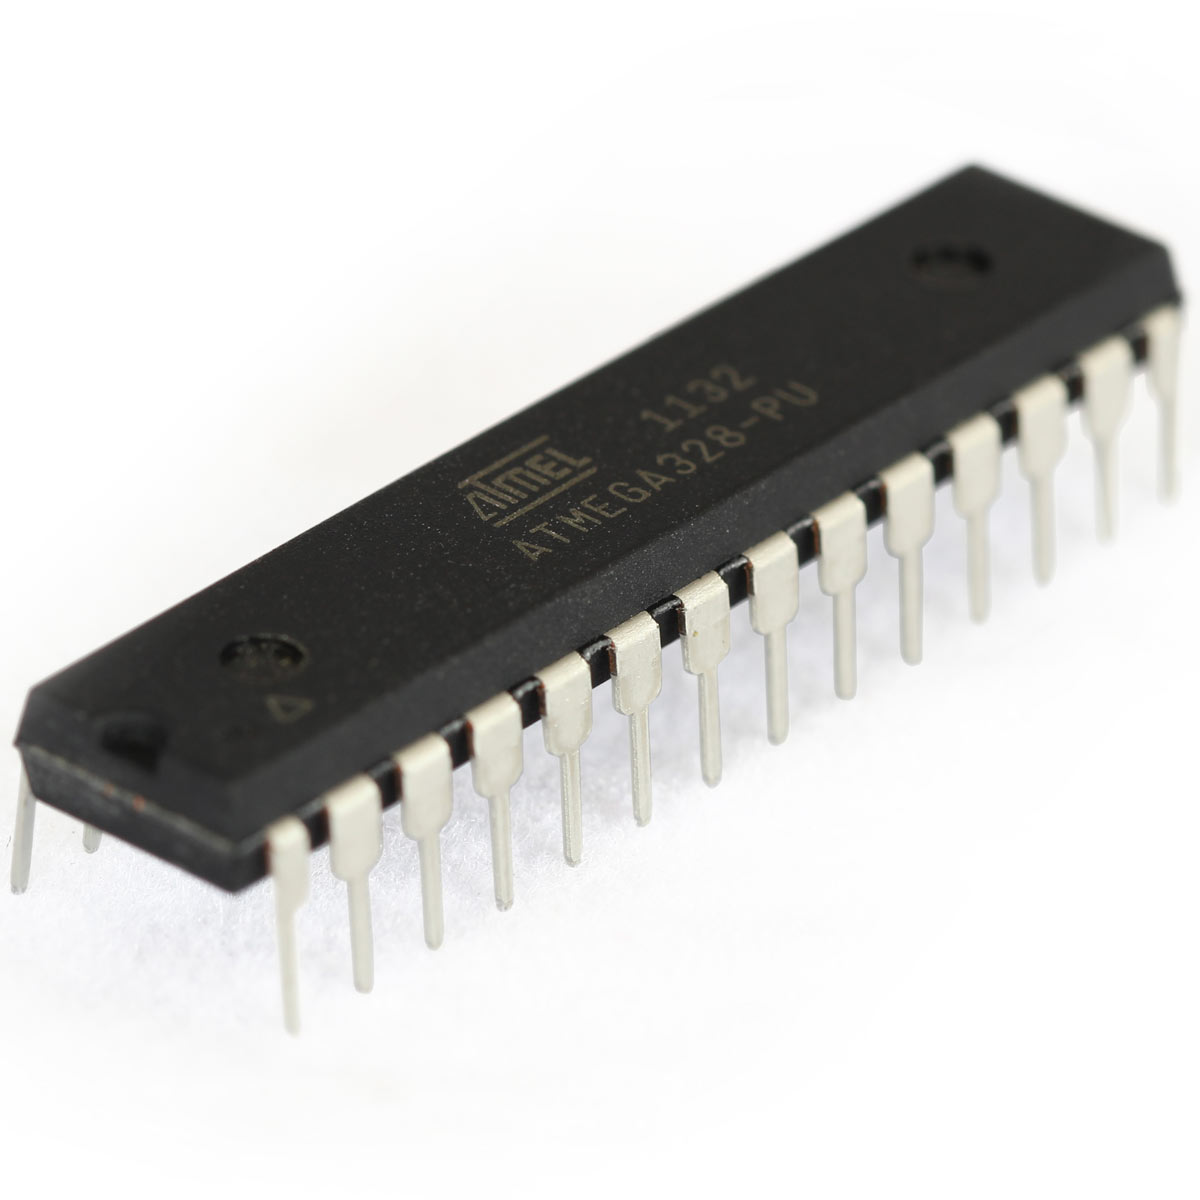
\includegraphics[width=0.3\textwidth]{Images/328p.jpg}
    \caption{ATmega 328p 28-SPDIP package }
\end{figure}

\begin{figure}
    \centering
    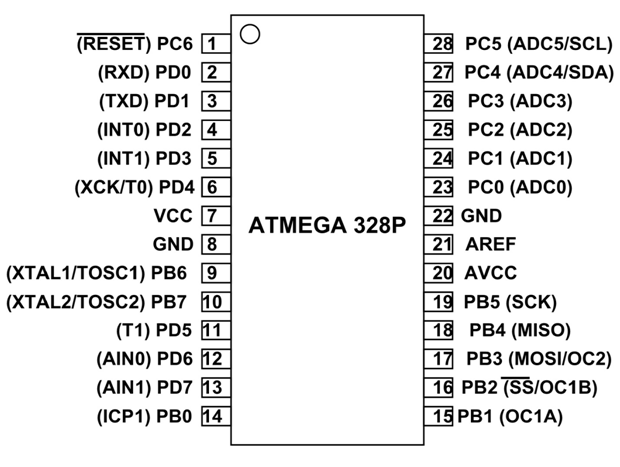
\includegraphics[width=0.3\textwidth]{Images/328p pinout.png}
    \caption{Pin Diagram }
\end{figure}

\subsubsection{Microphone}
The KY-037 module was selected as the microphone for our project. This module consists of a sensitive capacitance microphone and an amplifier circuit. The output of this module is both analog and digital. Only the analog output was used in our case. An image of KY-037 is shown in figure 3. 
\begin{figure}
    \centering
    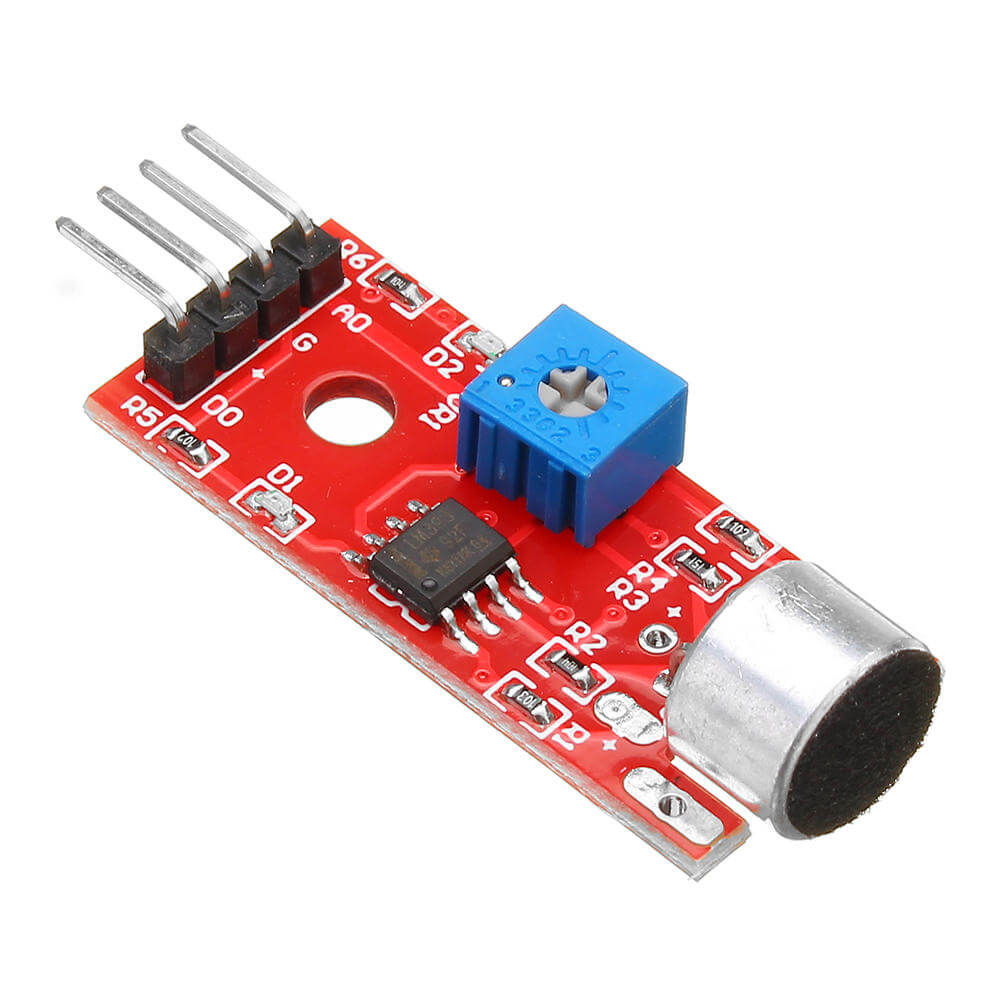
\includegraphics[width=0.3\textwidth]{Images/mic.jpg}
    \caption{KY-037 Microphone module}
\end{figure}

\subsubsection{SD Card Module}
We had the options to select USB Drive or SD card for storage purposes. But SD card was the item that met with our project requirements. Among SD card types we choose SD type because it was sufficient for our achieve our objectives.
An image of the SD card module is shown in figure 4.
\begin{figure}
    \centering
    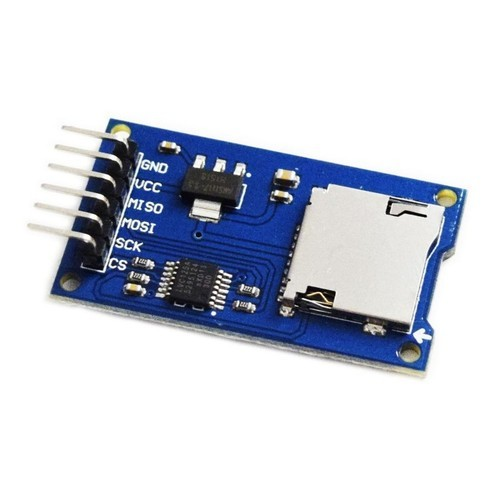
\includegraphics[width=0.3\textwidth]{Images/sd.jpg}
    \caption{SD Card Module}
\end{figure}

\subsubsection{LCD Display}
This display was selected due to its compliance to our requirements. The 16x2 LCD display was used in the 4-bit mode. An image is shown in figure 5.
\begin{figure}
    \centering
    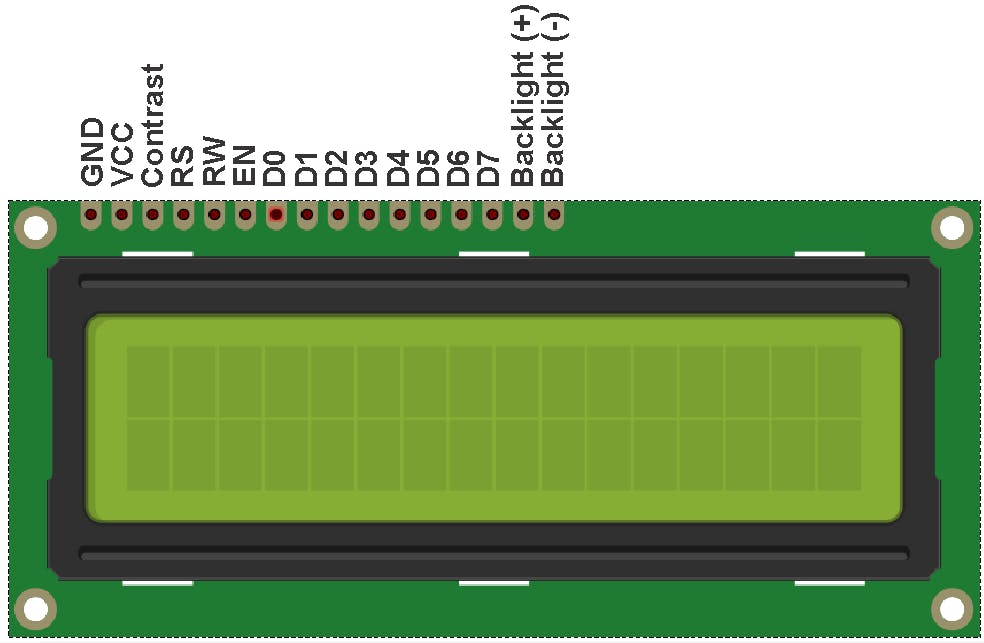
\includegraphics[width=0.3\textwidth]{Images/lcd.jpg}
    \caption{16x2 LCD Display}
\end{figure}

\subsubsection{Operational Amplifier}
A LM386\cite{386} operational amplifier is used in the speaker system as an audio amplifier.The main reason to use this amplifier specifically is the high gain of 200 from the amplifier and the availability of it.Here a potentiometer is also used in this amplifier circuit which can be used as a volume control to the output .The implementation of the operational amplifier is shown in figure 6.
\begin{figure}
    \centering
    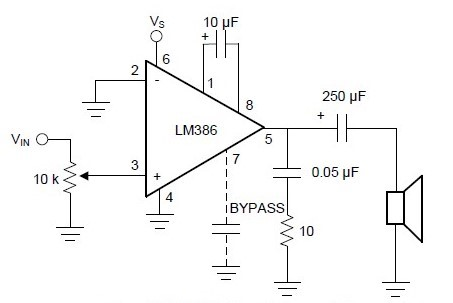
\includegraphics[width=0.3\textwidth]{Images/386.jpg}
    \caption{LM386 Circuit with 200 Gain}
\end{figure}

\subsubsection{Speaker}
A small 0.5W ,16$\Omega$ speaker is used along with the low pass filter and the amplifier circuit.A small speaker was used to make the prototype as small as possible. Figure 7 shows the speaker we have used for our prototype.

\begin{figure}
    \centering
    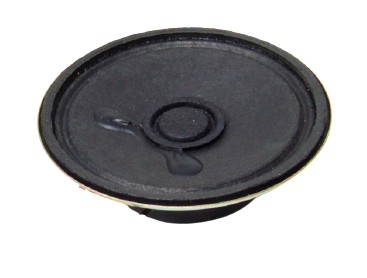
\includegraphics[width=0.3\textwidth]{Images/speaker.png}
    \caption{Speaker}
\end{figure}

\subsubsection{Regulator}
A LM7805 regulator\cite{7805} was used. This regulator is used to convert 9V power supply to 5V in which the circuit operates. see Figure 8.
\begin{figure}
    \centering
    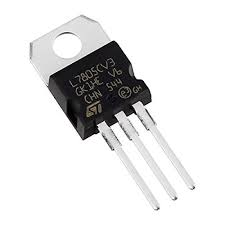
\includegraphics[width=0.3\textwidth]{Images/7805.jpg}
    \caption{LM7805 Voltage Regulator}
\end{figure}

\subsubsection{Other Components}
Table 1 listed the other components we have used except the components listed above.
    \begin{center}
        \caption{Table 1 - Other components}
        \begin{tabularx}{0.475\textwidth} { 
        | >{\raggedright\arraybackslash}X 
        | >{\centering\arraybackslash}X 
        | >{\centering\arraybackslash}X | }
        \hline
        Component & Value & Quantity \\
       \hline
       Oscillator & 16 MHz  & 1  \\
       \hline
       Push button & - & 4 \\
       \hline
       Slide switch & - & 1 \\
       \hline
       Resistor & 10 K$\Omega$ & 6 \\
       & 10K$\Omega$ & 5 \\
       & 8K$\Omega$ & 1 \\
       & 2 K$\Omega$ & 1 \\
       & 470 $\Omega$ & 1 \\
       \hline
       Potentiometer & - & 1 \\
       \hline
       Capacitor & 22pF & 2\\
       & 100nF & 3 \\
       & 10$\mu$F & 1 \\
       & 0.05$\mu$F & 1 \\
       & 250$\mu$F & 1 \\
       & 1$\mu$F & 2 \\
       \hline
       Battery & 9V & 1 \\
       \hline
       Battery socket & 9V & 1 \\
       \hline
       \end{tabularx}
    \end{center}
    
\subsection{Audio Input}
The voice signal obtained from the microphone module (see figure 9) is directed to the analog port of the microcontroller. At the initial stage the signal was directly given as a parameter to the record function of  the TMRpcm library present in Arduino  after scaling to 8-bits. In AVR custom functions were written to initialize and read the ADC. 128 was chosen as the ADC prescalar. Then 10-bit analog value was converted to 8-bit. As we have used a microphone module instead of a normal microphone, using a seperate low pass-filter is not necessary. In the Arduino platform, microphone was tuned in such a way that the audio input is properly received. To get the samples recursively, a while loop was used with required delay and to break the loop an external interrupt was attached to the enter button.
\begin{figure}
    \centering
    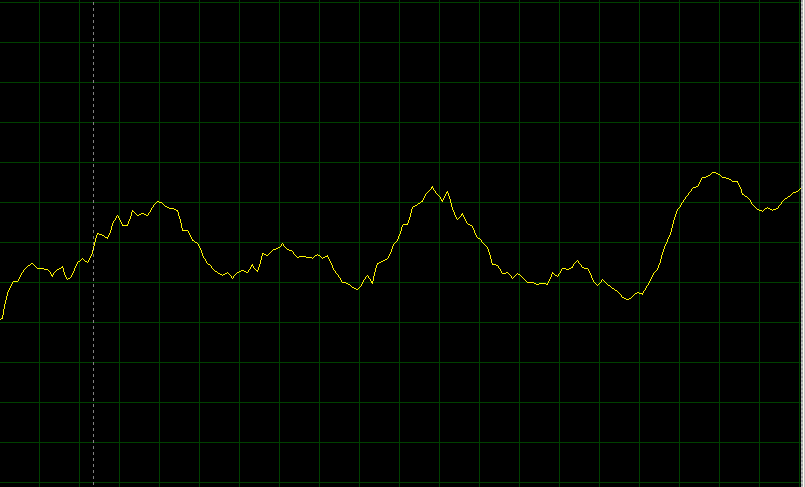
\includegraphics[width=0.475\textwidth]{Images/inputWave.PNG}
    \caption{Simulated input wave form}
\end{figure}

\subsection{Saving Audio}
%In the initial stage, we implemented our project on the Arduino platform. 
In the initial stage we used Arduino SD library to implement the communication between MCU and the SD. To establish an effective data transmission from the SD card we have to dedicate PB2 in  Atmega328p or D10 in Arduino Uno. Then we had the option to save data as a wav file or text file as we mentioned earlier. TMRpcm Arduino library was used to save data as a wav file. With the help of that library’s functions, we were able to directly write down the values to the SD Card. 
%We used an 8KHz sample rate for recording. Data retrieving and playback from the SD card are also done by using the TMRPCM library.

Then we used the text file method as an alternative method for the above method. In this method, we had to save analog input values to a text file. 
%Though the “analogRead” function in Arduino yields a value from 0 to 1023 we kept it in the range 0 to 255. 
We experienced a significant delay in the recording phase due to data write function from the SD library. Due to that reason, we decided to not to convert sample values to 8 bits and tried to reduce the delay as much as possible.  Then the sample values were converted to a text which is the length of 3 characters. Otherwise,as an example we won’t be able to differentiate three consecutive ‘1’s and ‘111’.

Due to the lack of built in libraries in the AVR platform, we had to use Arduino the SD library in the AVR platform also. So same procedures were implemented in this platform too. 

\subsection{File management}
"AUD(filenumber)" was chosen as the file naming format as "AUD00", "AUD01" and so on. At the arduino implementation a seperate text file was used to store the current audio file number. But later the current audio file number was stored in the EEPROM of the microcontroller. When displaying the files in the menu they were sorted in descending order. 

This voice recorder is capable of deleting selected file or deleting all files at once. In case of deleting all files the current file number goes to zero again. 

\subsection{Audio playback}
%Initially we used an arduino library TMRpcm to play a wav format file which is saved in the sd card.
After coding the playing of the wav file in Arduino, speaker part was simulated separately using the Proteus software. Here the output was generated using the PWM method by the TMRPCM library and the sampling frequency was set to 8KHz with 8 bit resolution. The speaker was implemented physically in an Arduino Uno for better manipulation of the audio output.

Then we chose several DACs like MCP-4725, MCP-4921, DAC0808  to implement the  DAC mode. After working with each DAC we chose the DAC0808 finally due to its low latency and higher accuracy.

For combining the parts of the voice recorder we used the PWM mode initially as it does not need special hardware. After making a combined simulation we were able to make a fully functional voice recorder setup in an Arduino Mega board.

%In implementing the voice recorder in AVR we decided to save the recorded file as a text file in the SD card.
Since at the AVR the text file method was used, the speaker part was designed to read the text file and to give the necessary output wave from.

In using a DAC to generate the output a timer interrupt was used in the code in which rises in regular time intervals with the frequency equal to the sampling frequency in which the sample value is written to the DAC0808.

Code was also written using the fast PWM mode of ATmega 328p. Here we created a PWM wave in 8KHz and created a loop which run in the same frequency to change the dutycycle of the wave according to the value of the samples to generate the output wave.

We implemented the fast PWM method in the final prototype (Simulated wave form is shown in figure 10). Here we used a low pass filter and the amplifier with the operational amplifier to get a clear and a louder output. The potentiometer of the amplifier is used as the volume controller of the voice recorder.

\begin{figure}
    \centering
    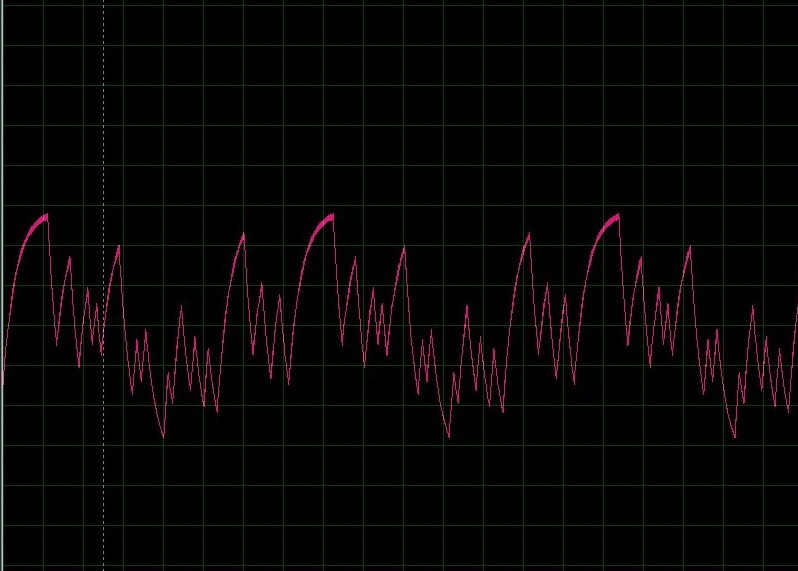
\includegraphics[width=0.475\textwidth]{Images/output.jpg}
    \caption{Simulated output wave form}
\end{figure}


\subsection{Audio Effect}
As our audio effect we decided to implement a frequency shifting. Same procedure in the audio playback is used and the PWM value was calculated according to eqs. (1).

\begin{equation}
    Xj(\omega-\omega_0) = e^{-j\omega_ot}x(t)
\end{equation}

Since the audio effect could not be differentiated properly from original audio a MATLAB code was written to observe the spectrum change that has occurred due to the changes done (See figure 11). 
\begin{figure}
    \centering
    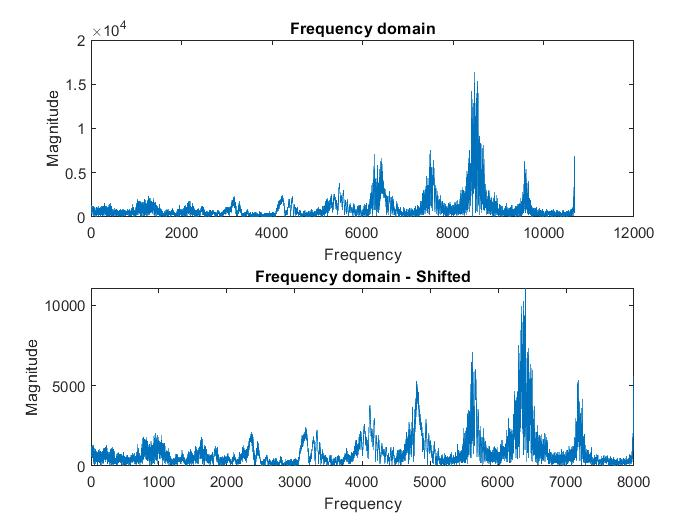
\includegraphics[width=0.475\textwidth]{Images/matlab.jpg}
    \caption{MATLAB Simulation}
\end{figure}

\subsection{Display and Menu}
As the first step, the menu and the display were implemented using the Arduino platform and was checked the functionality of the menu display using Proteus simulation. Liquid Crystal library was used for this purpose. The menu was made in such a way that there is a scrolling effect when the user moves up or down through the options present in the menu. A value is set to the variable position. This variable is updated whenever a button is pressed accordingly. The menu option that is to be displayed in the screen changes correspondingly.

Next the LCD display was required to be converted into AVR platform. The LCD was connected to the ATmega328p microcontroller using six pins, one for Register Select (RS), one for Enable and four pins for data transmission. In the four-bit mode the eight bit ASCII value has to be divided into nibbles and sent to the display. The separated nibbles, lower nibble and higher nibble are sent through the same calculations. The higher nibble is sent first followed by the lower nibble. The hexadecimal values of the commands are also sent in a similar manner. A library specific for the  project for the LCD was made. The options were given as character arrays, so that the print function in the LCD library can select one character from the array at a time and send the command to the LCD to display the character. Menu position functions were defined in the algorithm of the menu so that the LCD can display required menu options. 

Four buttons were used to control the menu. They were Up, Down, Enter and Back. The  user can scroll up or down the options using the up and down buttons and select any option using the enter button.  Each button is connected through a pull down resistor of 10K$\Omega$ to the ground.


\subsection{Power circuit}
9V battery is used as the power source. Then a LM7805 voltage regulator is used to convert 9V to 5V. At the input side a 1$\mu$F capacitor is used to catch unwanted signal like transients and other noises. Another 1$\mu$F capacitor is used at the output to filter unwanted oscillations. 

\subsection{PCB Design}
The schematic (Appendix 1) of the circuit was drawn first and the PCB (Appendix 2 and 3) was designed accordingly using Altium. The PCB was made small as much as possible. Power lines were made more thick than the signal lines. Lines were routed in the top and the bottom layer. The signal lines were routed at a thickness of 0.254mm and the power lines were routed at the thickness of 0.35mm. 

\subsection{3D Enclosure}
The PCB designed using Altium was exported to Solidworks as a 3D step file. Then external parts such as microphone module, slide switch, SD card, speaker, LCD, battery socket and button knobs were imported to the 3D assembly.
Next the bottom part of the enclosure and the top part of the enclosure were designed. Openings for microphone, SD card, slide switch and battery socket were placed in the bottom part while openings for LCD, speaker and the knobs were placed in the top part of the opening. The top part and the bottom part were connected using fasteners (Appendix 4 and 5).


\section{Results}
The microphone module, SD card, LCD display and the menu worked properly without any failure. The buttons did not have any bouncing effect. The expected scrolling effect of the menu worked properly. The file number variable saved in the EEPROM was updated automatically without any mistake. This was observed by properly monitoring the file operations done in the voice recorder. The sorting algorithm used to sort the files in the descending order worked ideally. The above results were observed using the breadboard prototype (See figure 12). 

The only drawback was the low quality of the sound coming out from the speaker. The sound could not be heard properly. 

Special functions of the final code have been attached to appendix 6 to 11. 

To see the GitHub repository: \\
\url{https://github.com/K-Thanushan/Simple-Voice-Recorder}

\begin{figure}
    \centering
    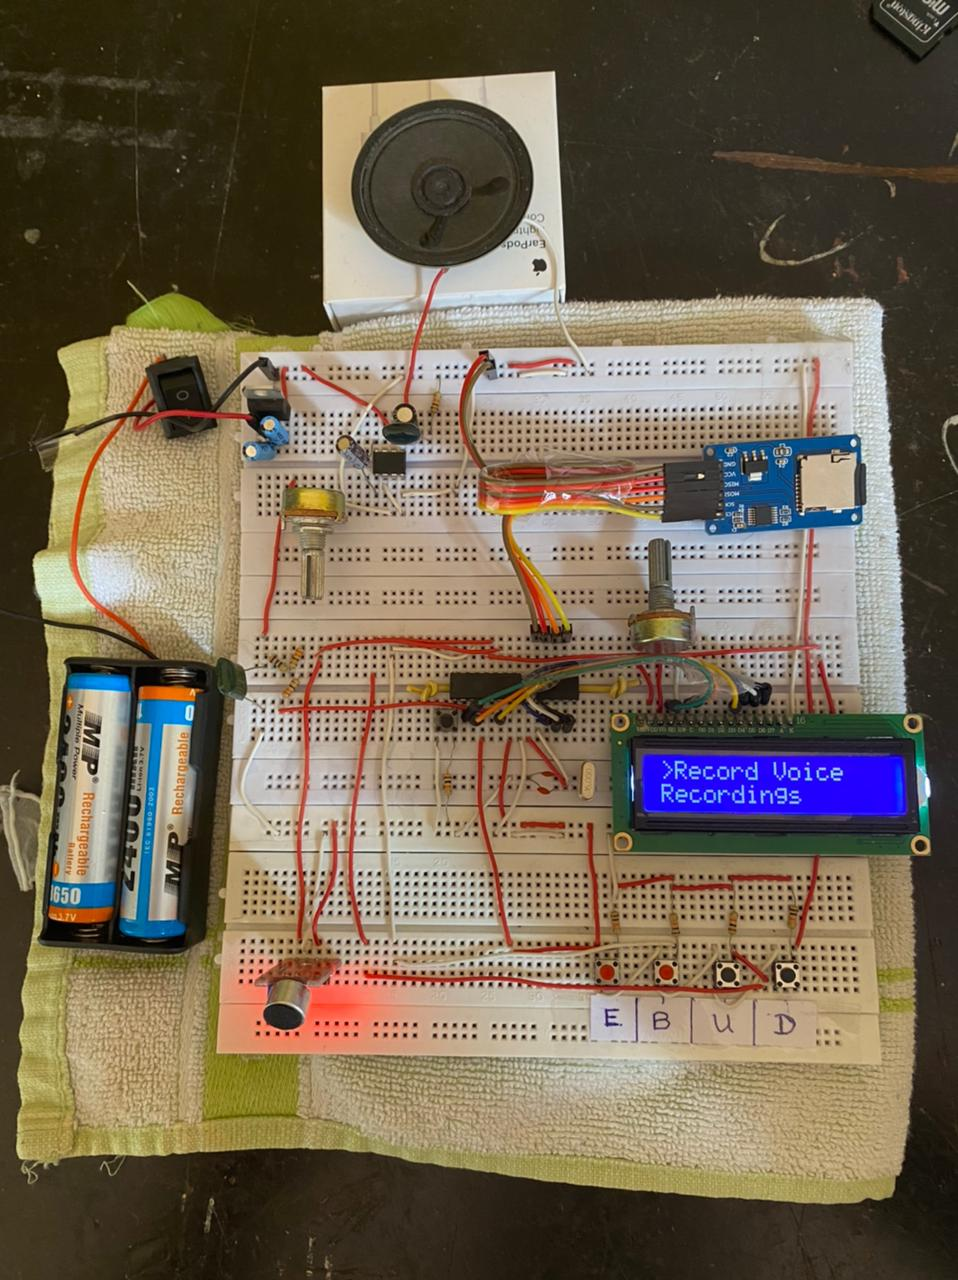
\includegraphics[width=0.475\textwidth]{Images/imple.jpeg}
    \caption{Breadboard Implementation}
\end{figure}

\section{Discussion}
Each and every part of the voice recorder was separately implemented and then it was combined.Initially ATmega2560 was selected for combining the code. The prototype was successful in the proteus simulation and on the Arduino Mega board. Later it was found that it is difficult to implement the prototype using the above microcontroller on a breadboard since ATmega2560 is a SMD(Surface Mount Device). Therefore we had to shift to ATmega328p. The same code implemented in ATmega2560 was implemented in ATmega328p but the memory of the latter was not enough for the code to be executed. Therefore certain libraries had to be changed.As a first step Liquid Crystal Library was replaced by our own tailor made LCD Library in AVR platform. Also we had to change our approach from using wave file format analysis using TMRpcm to analyse using text file format of the recording.

We decided to use a 16MHz external oscillator instead of 8MHz internal oscillator to maintain a higher clock rate and a higher accuracy. However maintaining a constant sampling rate throughout the whole process was one of the major issue we faced during the project. A significant amount of time was taken to write a sample to the SD card. Therefore we used our own method to maintain a nearly constant sampling rate. We checked the time taken for a single loop and made a delay for the remaining time needed to obtain the sampling period.

As we mentioned in the above paragraph we had two options to store the the audio input. One option was the text file format and the other one was the wave file format. In both options there were some advantages and disadvantages that affected our project in a serious manner. The wave file format is a more quality option. But the memory issue appeared caused us to abandon the above format. So the text file was the obvious option for the storing purpose. On the other hand the quality of the output was reduced in a considerable amount. Due to the unavailability of a DAC module this was changed to get the output using PWM method. In simulations the simulation of the speaker was hard to execute as the run time of the Proteus software was not equal to the real time causing several problems. A lot of adjustments were done with the low pass filter and the amplifier even to get the output sound to the stage at present.

When the project was advanced in to the AVR platform, there was an another issue for the SD card.The difficulty to find a built in library for the SD card module caused to use the Arduino SD library for the AVR platform also. 

A certain latency is present when the LCD is operating in the 4-bit mode when compared to the 8 bit mode but it the four bit mode uses only four pins for data transfer whereas the 8 bit mode uses 8 pins. Therefore the 4 bit mode is chosen for the project since it uses less number of pins of the microcontroller than the eight bit mode.Initially the recording file list was defined as a two dimensional character array. But there were some errors since the elements of the list cannot be accessed. The final code was a combination of both Arduino and AVR platforms. Therefore the file list was defined as a list of strings. The menu position functions were modified to accept strings and then the accepted strings were converted into character arrays using "toChar" functions and was passed to the print function of the LCD library. The bouncing effect created by pressing the button is rectified using a delay of 250ms. When considering the algorithm of the menu the position variable has to be handled carefully since that variable decides path of the menu. 


\section{Acknowledgement}
We would like to thank each and every person who has helped us even in a very small manner in order to achieve good results in this project. We would like to specially thank Mr. Thamidu Pathirana who was our project supervisor. He motivated us to learn the extra subjects required for this project ourselves. He also helped us in clearing our doubts and ambiguities regarding the project. 

\addcontentsline{toc}{section}{Reference}
\bibliographystyle{IEEEtran}
\bibliography{ref}

\onecolumn
\begin{figure}
\section{Appendices}
\subsection{Appendix 1 - PCB Schematic}
    \begin{subfigure}{\textwidth}
    \centering
    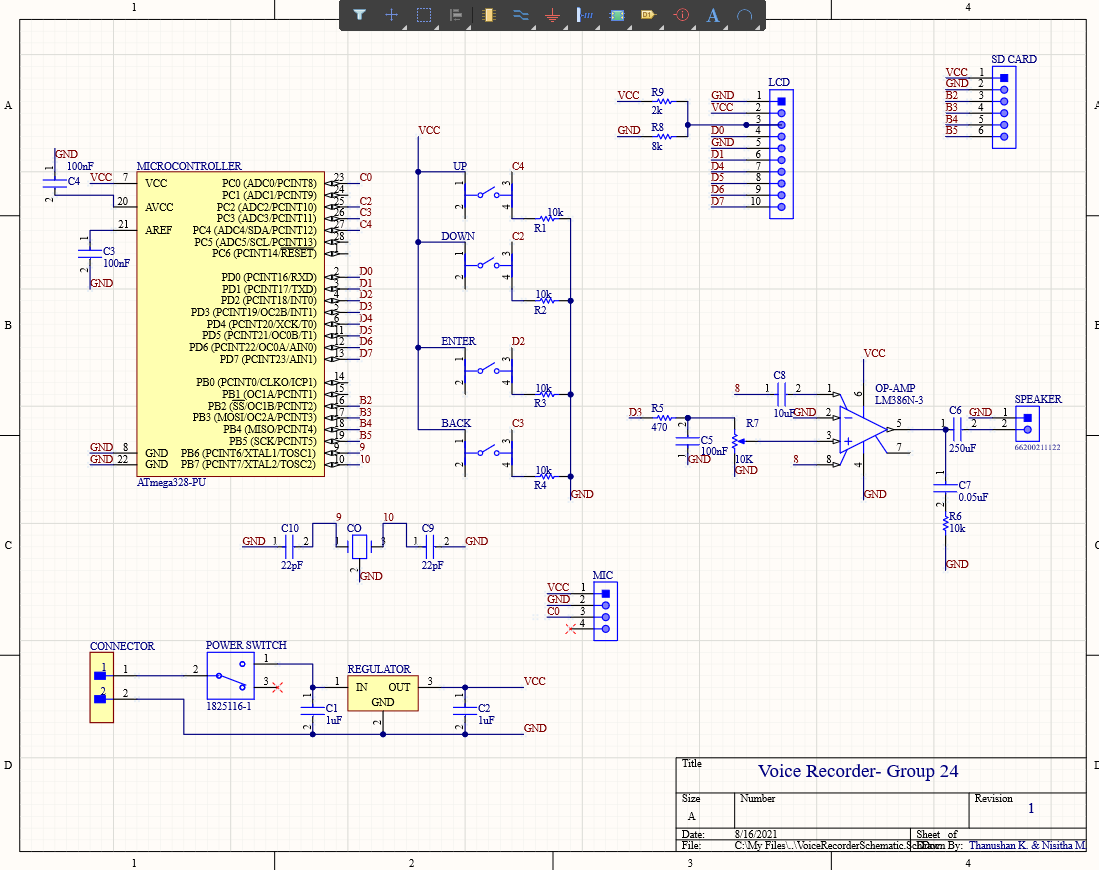
\includegraphics[width=1\textwidth]{Images/sch.png}
    \end{subfigure}
\subsection{Appendix 2 - PCB Routing}
    \begin{subfigure}{\textwidth}
    \centering
    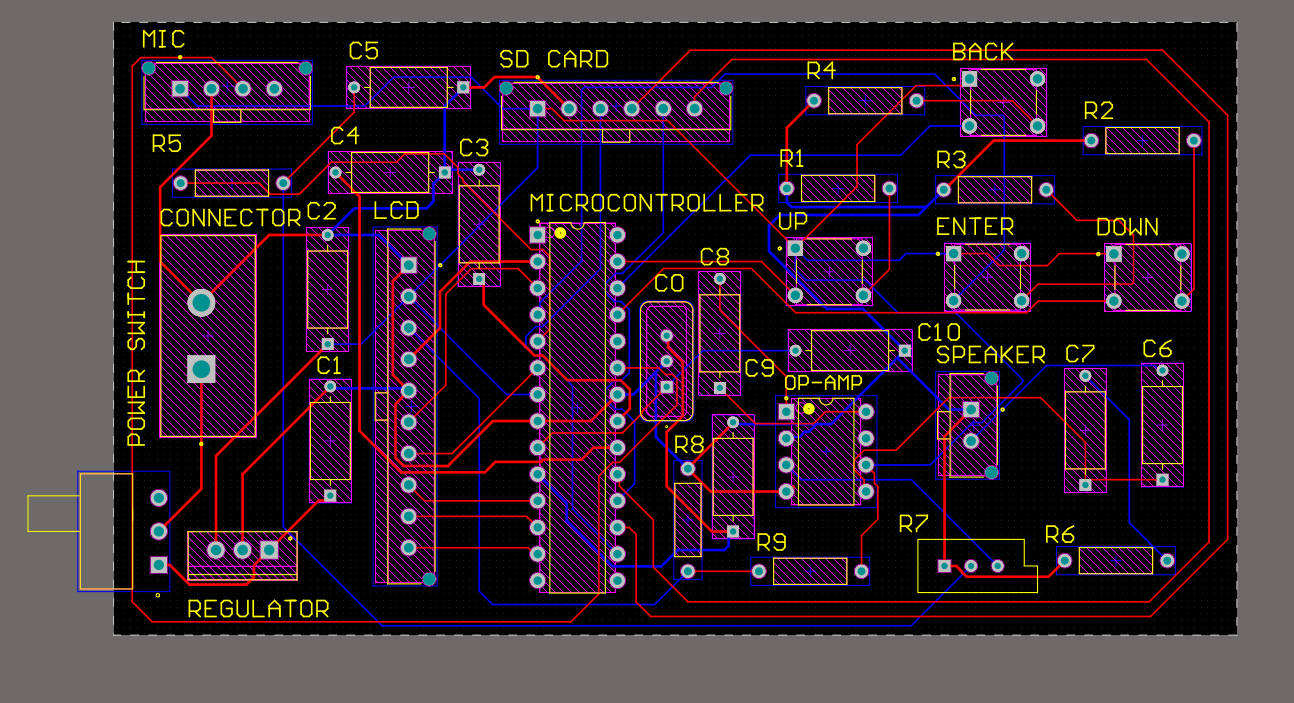
\includegraphics[width=1\textwidth]{Images/route.png}
    \end{subfigure}
\end{figure}

\begin{figure}
\subsection{Appendix 3 - PCB 3D View}
    \begin{subfigure}{\textwidth}
    \centering
    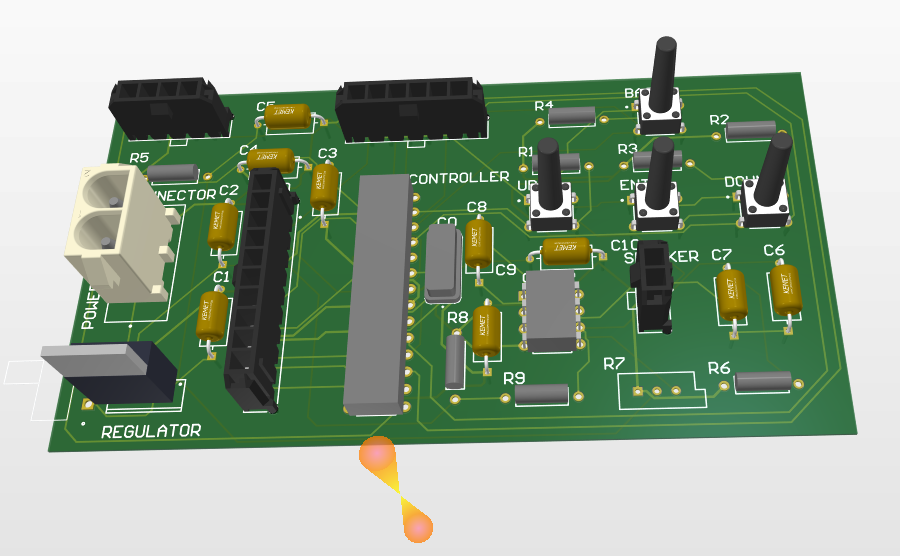
\includegraphics[width=1\textwidth]{Images/3D.png}
    \end{subfigure}

\subsection{Appendix 4 - Enclosure Design}
    \begin{subfigure}{\textwidth}
    \centering
    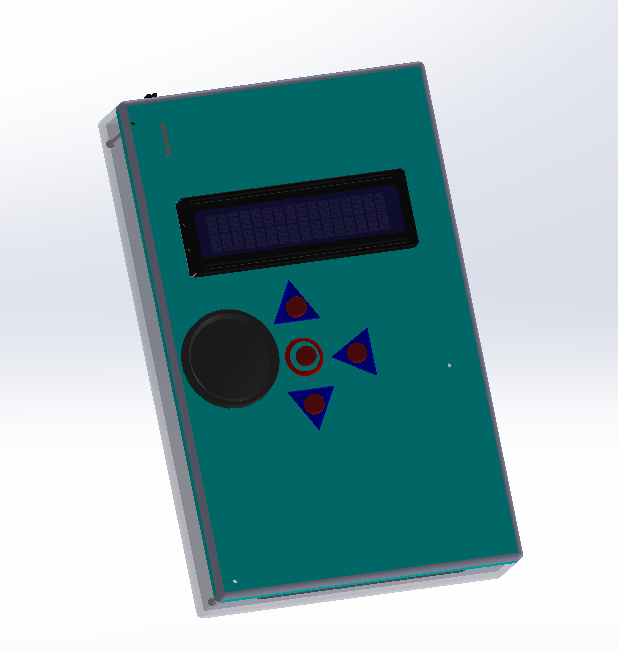
\includegraphics[height=0.7\textwidth]{Images/encl full.png}
    \end{subfigure}
\end{figure}

\begin{figure}
\subsection{Appendix 5 - Seperated Parts }
    \centering
    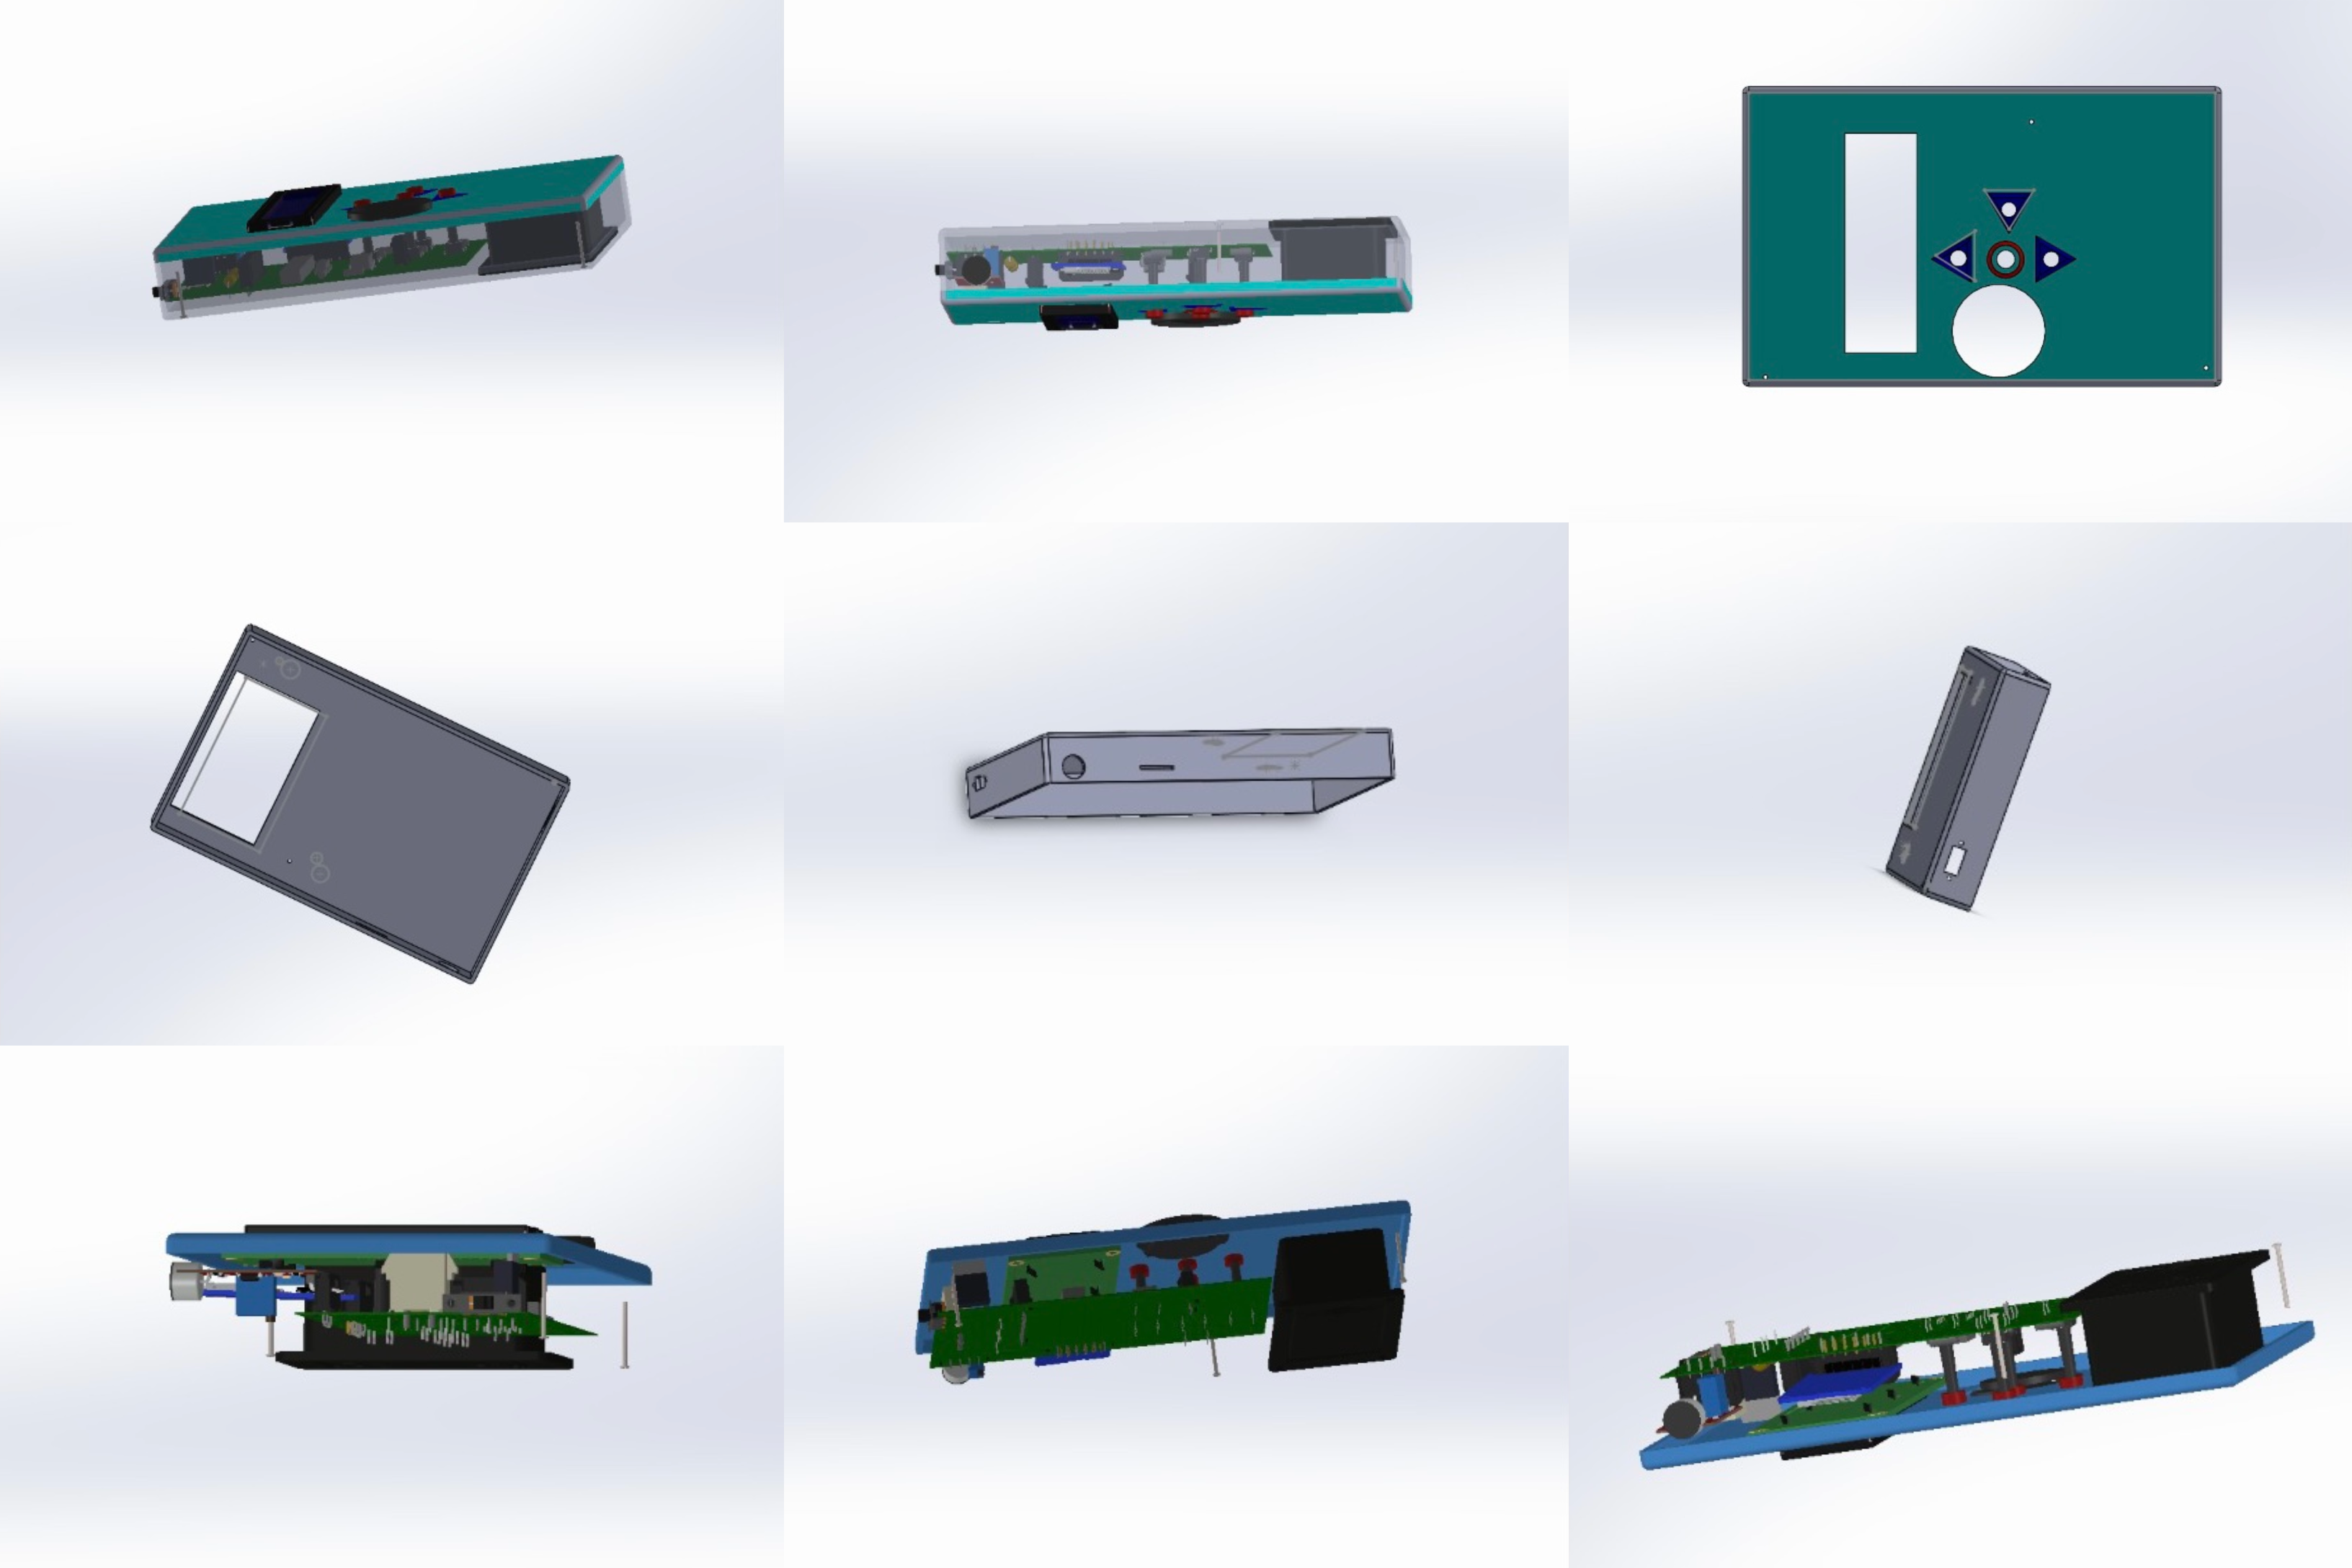
\includegraphics[width=1\textwidth]{Images/encl.png}
\end{figure}
\newpage

\begin{figure}
\subsection{Appendix 6 - LCD Library}
    \begin{subfigure}{\textwidth}
    \centering
    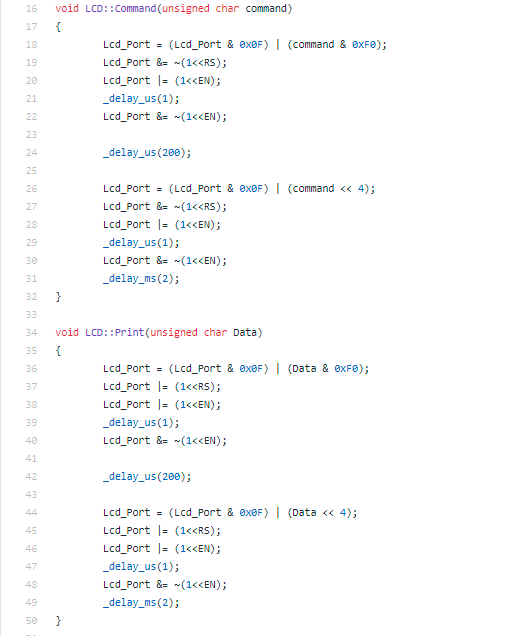
\includegraphics[width=1\textwidth]{Images/LCD_Lib_1.png}
    \end{subfigure}
\end{figure}
\begin{figure}
\subsection{Appendix 7 - Menu Position}
    \begin{subfigure}{\textwidth}
    \centering
    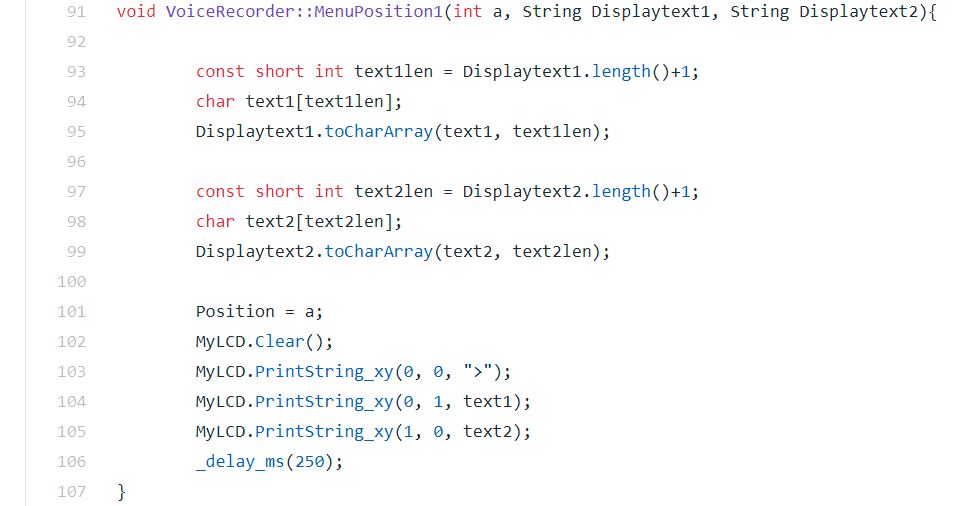
\includegraphics[width=1.2\textwidth]{Images/Menu_2.png}
    \end{subfigure}    
    \subsection{Appendix 8 - Analog Input}
    \begin{subfigure}{\textwidth}
    \centering
    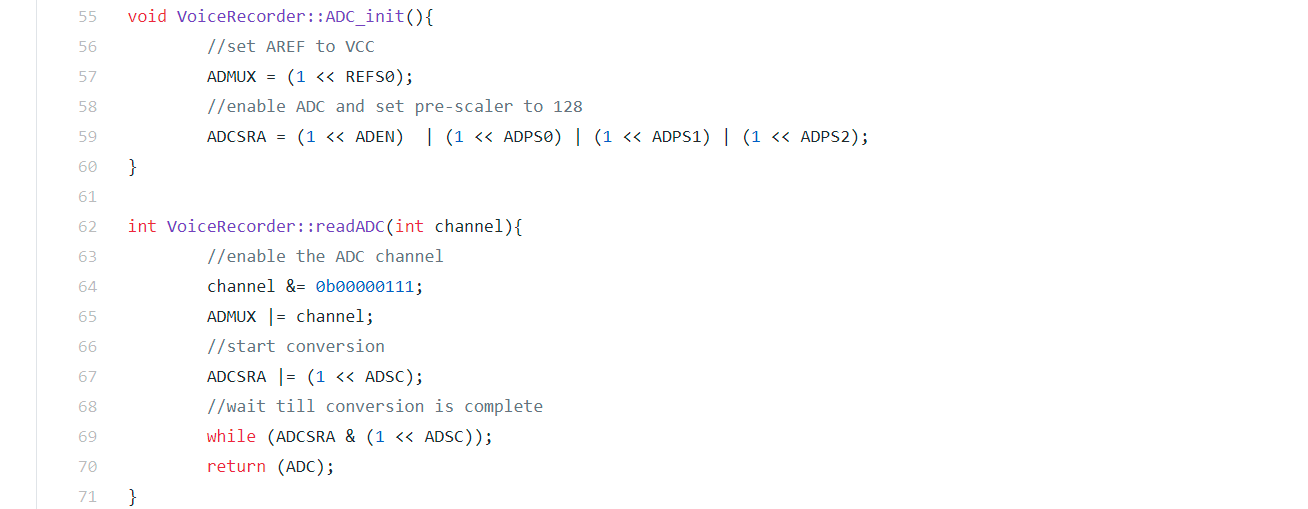
\includegraphics[width=1.5\textwidth]{Images/ADC_3.png}
    \end{subfigure}    
\end{figure}

\begin{figure}
\subsection{Appendix 9 - Start Recording}
    \begin{subfigure}{\textwidth}
    \centering
    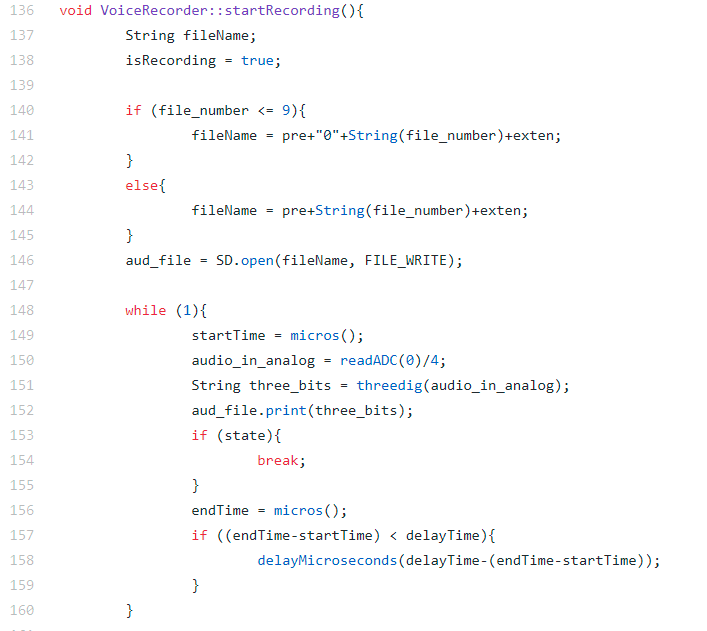
\includegraphics[width=0.85\textwidth]{Images/start_4.png}
    \end{subfigure}    
    
    \begin{subfigure}{\textwidth}
    \centering
    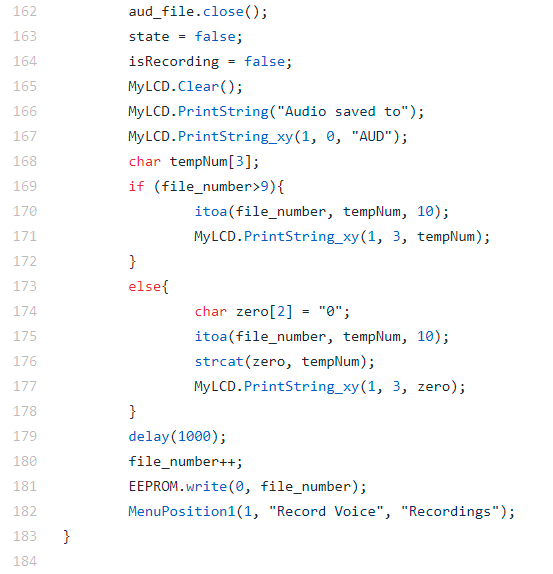
\includegraphics[width=0.75\textwidth]{Images/start_5.png}
    \end{subfigure}    
\end{figure}

\begin{figure}
\subsection{Appendix 10 - Start Playback}
    \begin{subfigure}{\textwidth}
    \centering
    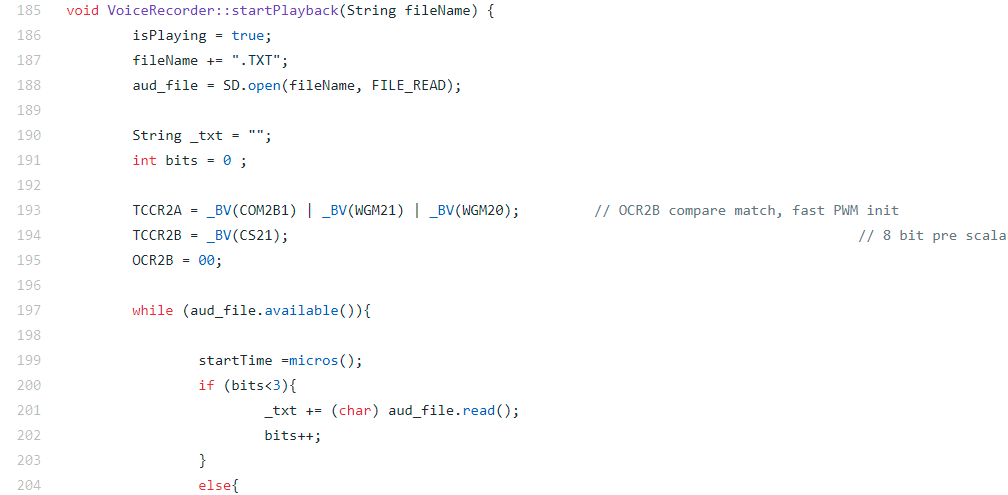
\includegraphics[width=1.2\textwidth]{Images/play_5.png}
    \end{subfigure}    
    
    \begin{subfigure}{\textwidth}
    \centering
    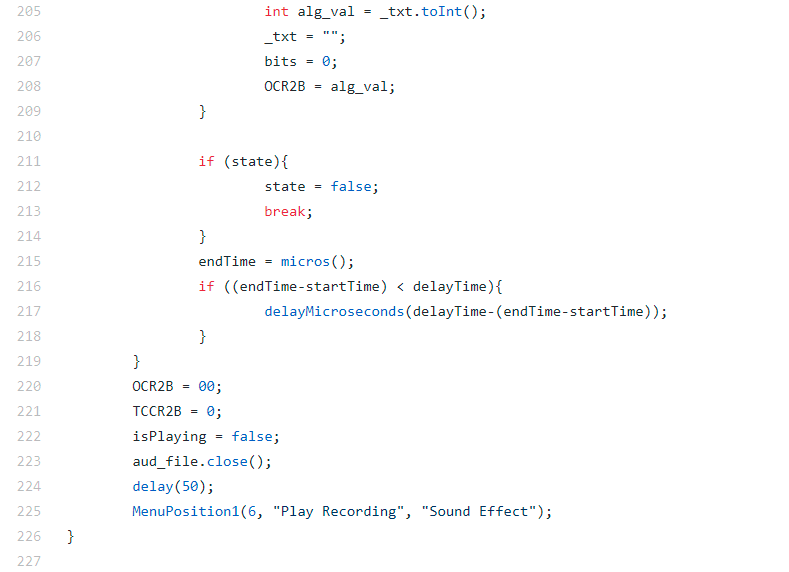
\includegraphics[width=0.95\textwidth]{Images/Play_6.png}
    \end{subfigure}    
\end{figure}

\begin{figure}
\subsection{Appendix 11 - Arduino Code }
    \centering
    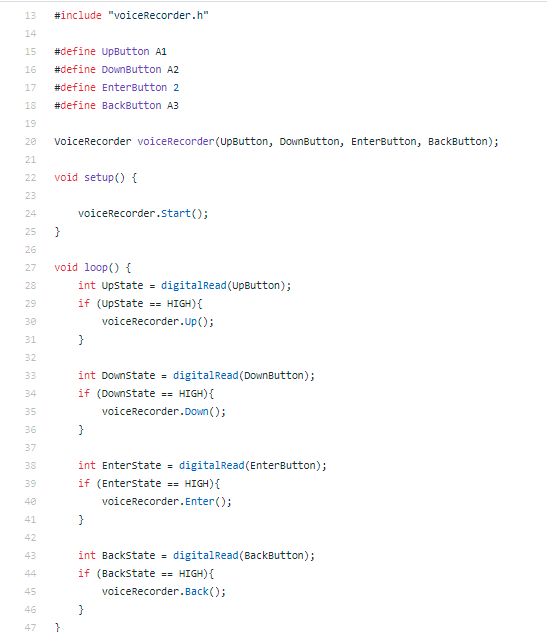
\includegraphics[width=1\textwidth]{Images/arduino.png}
\end{figure}

\end{document}

